One example of the dochotomy between an MPs voting patterns and their community work concerns former University of Edinburgh student Ian Murray \cite{ian-murray}, who has been the MP for the Edinburgh South constituency since the UK 2010 general election. 
In 2015, Hearts of Midlothian football club, which was founded in XXX, and which is one of the two football professional clubs in Edinburgh, faced closure following the bankruptcy of its Russian owner, XXXX.
As a consequence of his role as the local MP, Ian Murray was asked by supporters of the club to liase with the club's official receivers.
Over several years, his work led to a supports buyout the club, which is now the only football club in the Scottish (or, indeed, the English) Premier League to owned by the supporters.
Ian Murray was subsequently interviewed \cite{ian-murray-bbc} on the BBC Parliametrary channel \cite{bbc-parliament} with regard to a book he wrote, This is our story \cite{ian-murray-this-is-our-story}, describing his work helping the supporters of the football club.

\begin{figure}[h]
  \centering
  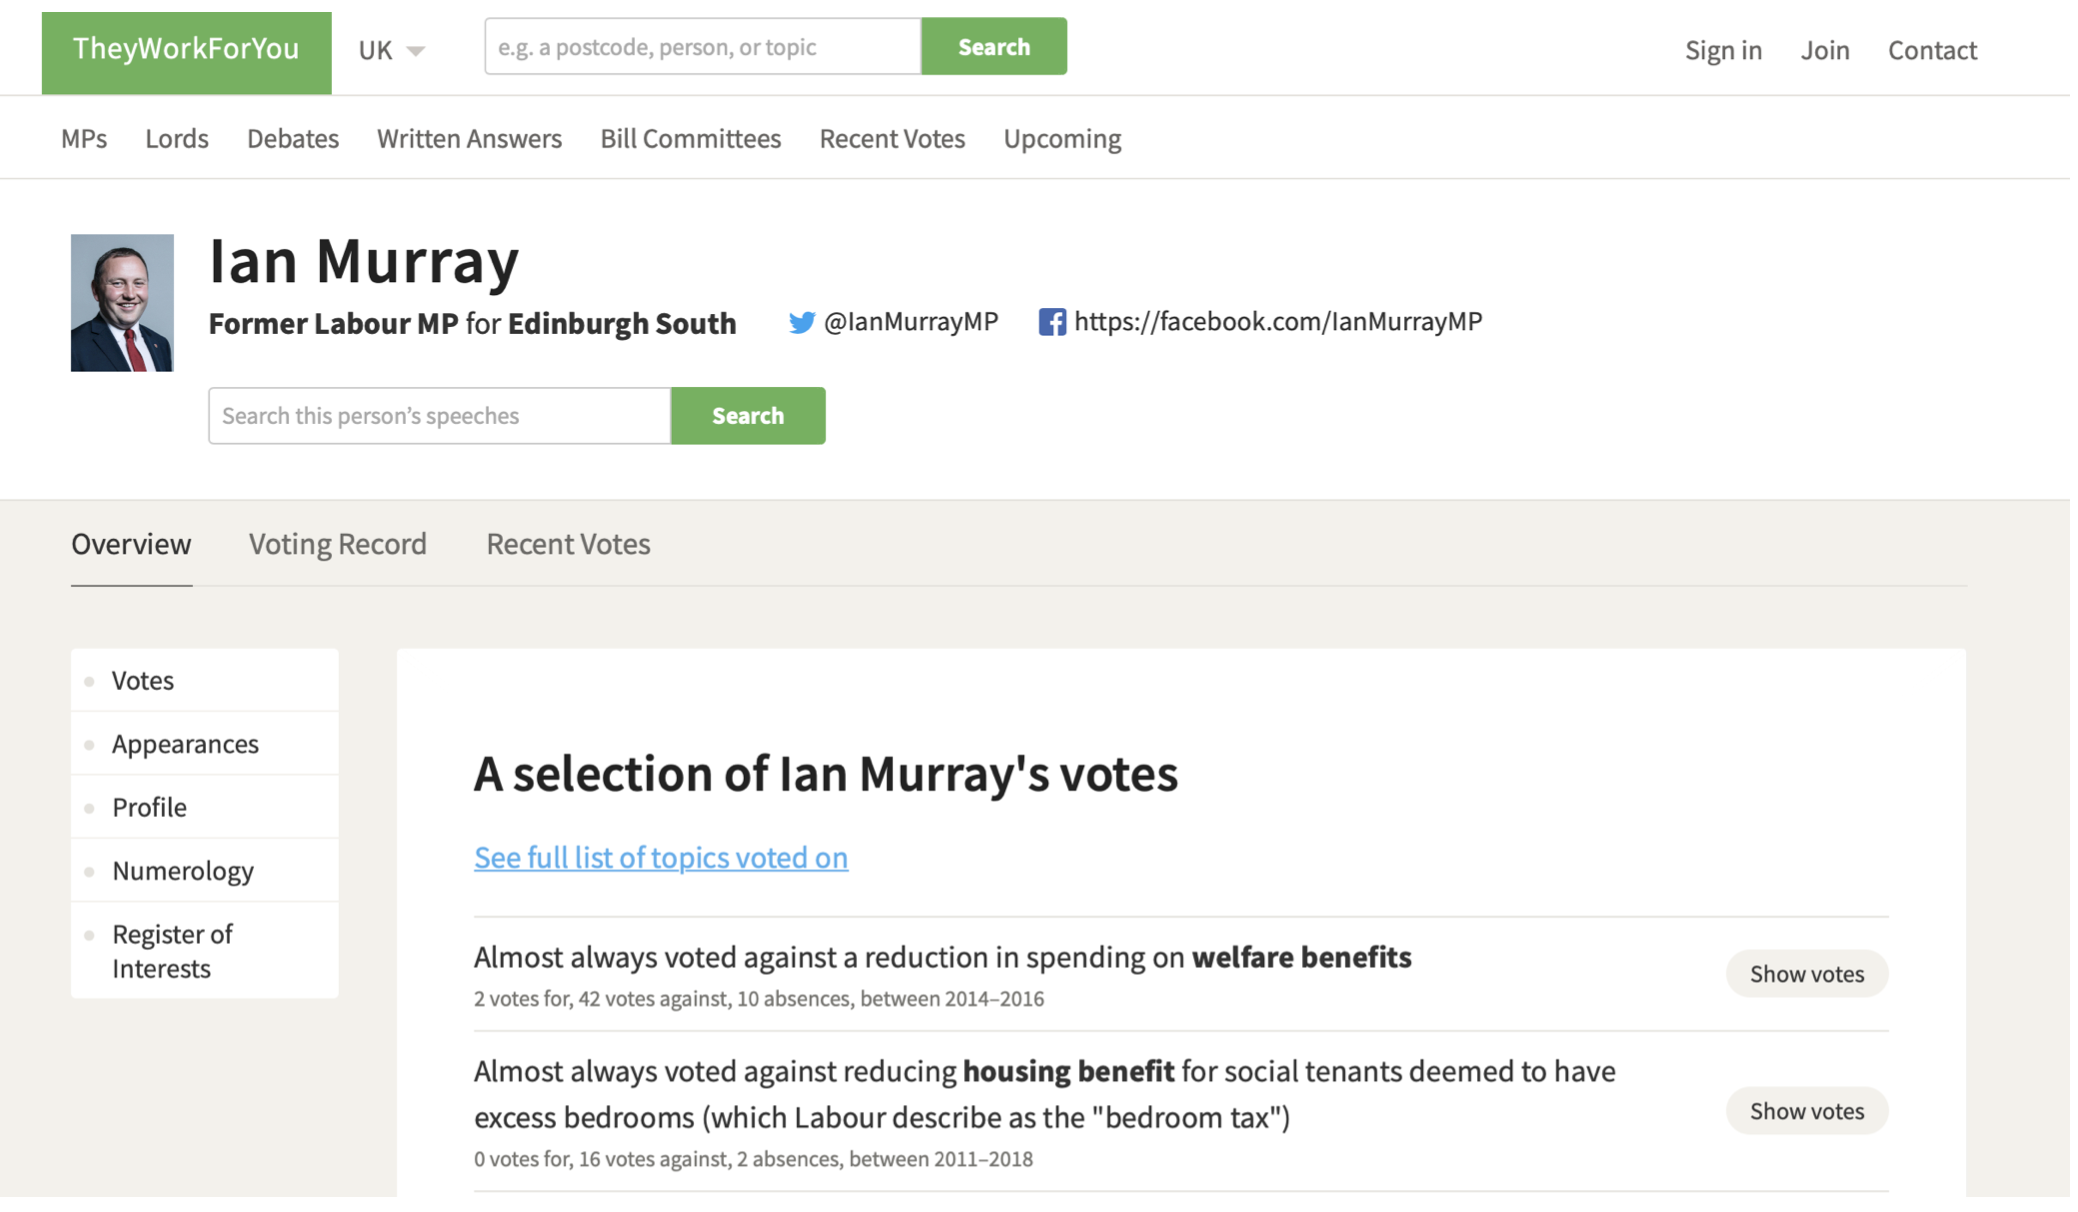
\includegraphics[scale=0.3]{images/they-work-for-you-ian-murray}
  \caption{They Work for You page for MP Ian Murray}
  \label{fig:they-work-for-you-ian-murray}
\end{figure}

However, while Ian Murray’s involvement came about because of his role as an MP, it did not involve any specific questions in the commons.
Consequently, is not described by the aggregated data on his They Work for You page, as can be seen from the screen shot within Figure \ref{fig:they-work-for-you-ian-murray}.